\chapter{电力系统的脆弱性仿真实验与量化分析}
\label{cha:quantiAnaly}

\section{引言}
\label{sec:index5}
依据第四章所建立的电网脆弱性量化评价模型,本章以$IEEE118$标准电网为例,在系统模型的基础上,采用静态分析法研究不同攻击策略对电网结构脆弱性的影响,找出最佳的攻击策略,并验证电力系统的网络特性。
以$IEEE39$标准电网为例,分别进行仿真实验研究电力系统的结构脆弱性和状态脆弱性,最后得到系统综合脆弱性评价结果,并与其它评价模型进行对比,验证本文所建立的评价模型的科学性。
\section{基于复杂网络模型结构脆弱性实验验证分析}
\label{sec:modelIntroduce}

\subsection{电网结构脆弱性研究方法}
\label{sec:modelIntroduce}
电网作为一个复杂的人造网络,存在一些固有的缺陷或薄弱环节,当这些薄弱环节遭到破坏时,由于电网节点间的连通性,可能会导致电网运行失稳,引发电网大面积瘫痪。在结构上看,这些缺陷或薄弱环节可视为
电网的脆弱环节,因此电网脆弱环节的脆弱程度可以表征电网结构脆弱性。

从复杂网络的角度来看,研究电网结构脆弱性的基本方法为通过移除部分节点或线路来考察电网结构和功能的影响程度。电网结构脆弱性的研究方法分为静态分析法和动态分析法,其主要区别在于移除节点或线路
后是否考虑所引起的级联反应。静态分析法通过不同的电网攻击策略,分析其对电网结构连通性及传输效率的影响程度,不考虑节点或线路移除后引起的级联反应。动态分析法则考虑的是节点或线路移除后潮流分布
变化所引起的级联反应,通过建立连锁故障模型来模拟电网结构性能的动态变化。由于本文对电网结构脆弱性的重点在于识别系统的薄弱环节,选取最优攻击策略,所以在研究方法上,采用静态分析法。 

\subsection{指标选取及元件攻击策略的制定}
\label{sec:modelIntroduce}
为识别电力系统的脆弱环节并找到最优的攻击策略,需要制定电网的攻击策略以及选取电网整体性能指标,从电网结构拓扑方面考虑,网络传输效率是用于描述电网能量传输的重要性能指标。为此,本文选取第二章所述
的网络平均传输效率$E_{mean}$作为电网结构性能评价指标。

在第三章中,通过对结构脆弱性的研究,得到电气度、电气介数和$PageRank$值这三个指标作为结构脆弱性指标,为比较这三个指标对于电网结构性能的影响程度,分别按照式\ref{equ:chap3:index1},式\ref{equ:chap3:cb1}
和式\ref{equ:chap3:Index3}计算$IEEE118$算例中各节点的电气度、电气介数$PageRank$值,并将各节点的计算结果进行排序。下面将围绕电气度、电气介数$PageRank$值这三个指标指定攻击策略,观察比较
电网结构性能指标的变化情况,并引入随机节点攻击策略作为实验对比。具体策略如下:

$(1)$随机节点攻击策略——每次随机移除1个节点,移除比例为30$\%$,仿真100次,取性能指标结果的平均值;

$(2)$电气度节点攻击策略——每次移除电气度值最大的节点,移除比例为30$\%$,记录每次的性能指标仿真结果;

$(3)$电气介数节点攻击策略——每次移除电气介数值最大的节点,移除比例为30$\%$,记录每次的性能指标仿真结果;

$(4)$$PageRank$值节点攻击策略——每次移除$PageRank$值最大的节点,移除比例为30$\%$,记录每次的性能指标仿真结果;



\subsection{实验仿真与分析}
\label{sec:modelIntroduce}
本文采用的$IEEE118$标准算例数据见附录A所示,其中各节点电气度、电气介数和$PageRank$值计算结果,分别如图\ref{fig:electricDu118},\ref{fig:nodeBetween118}和\ref{fig:pagerank118}所示,
实验结果数据见附录B。
\begin{figure}[H] % use float package if you want it here
    \centering
    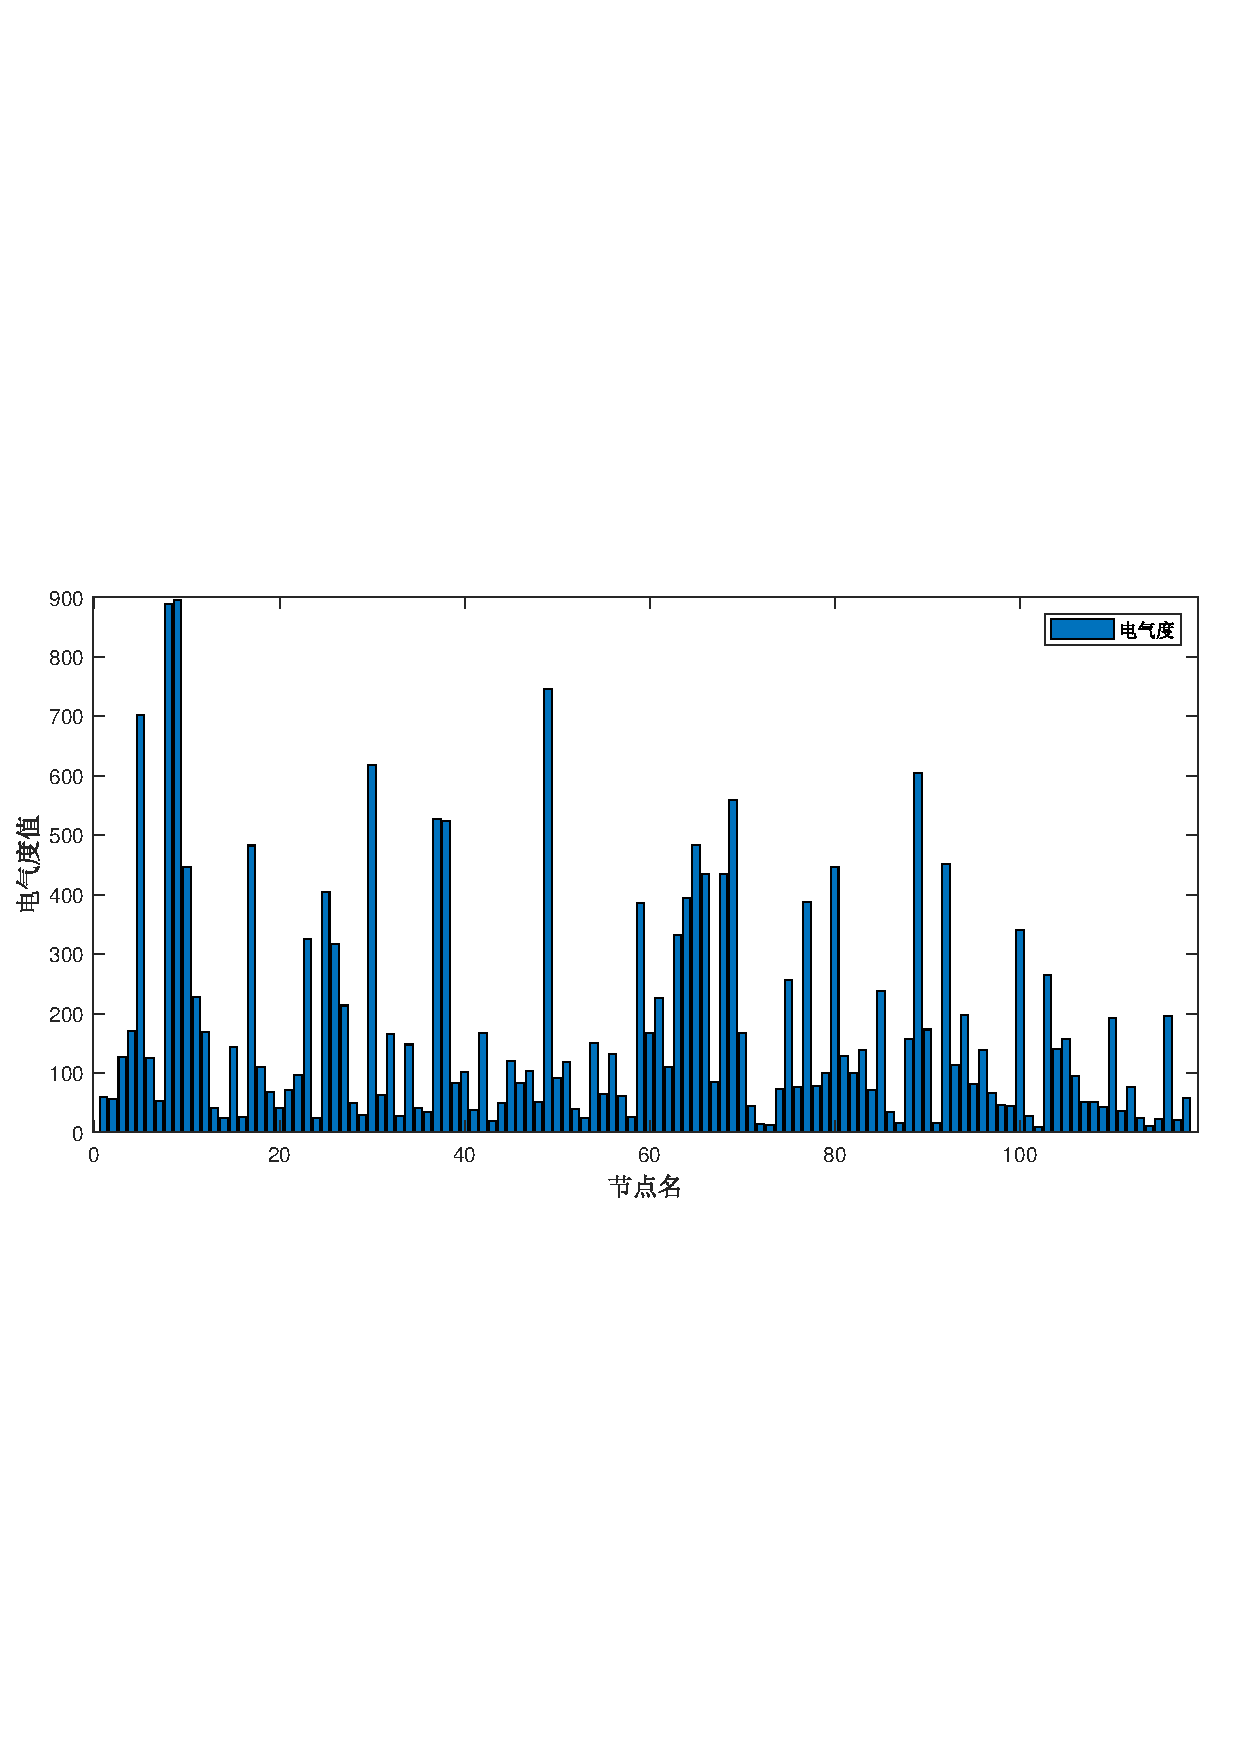
\includegraphics[width=14cm,height=7cm]{electricDu118.pdf}
    \caption{$IEEE118$节点电气度计算结果图}
    \label{fig:electricDu118}
  \end{figure}
\begin{figure}[H] % use float package if you want it here
    \centering
    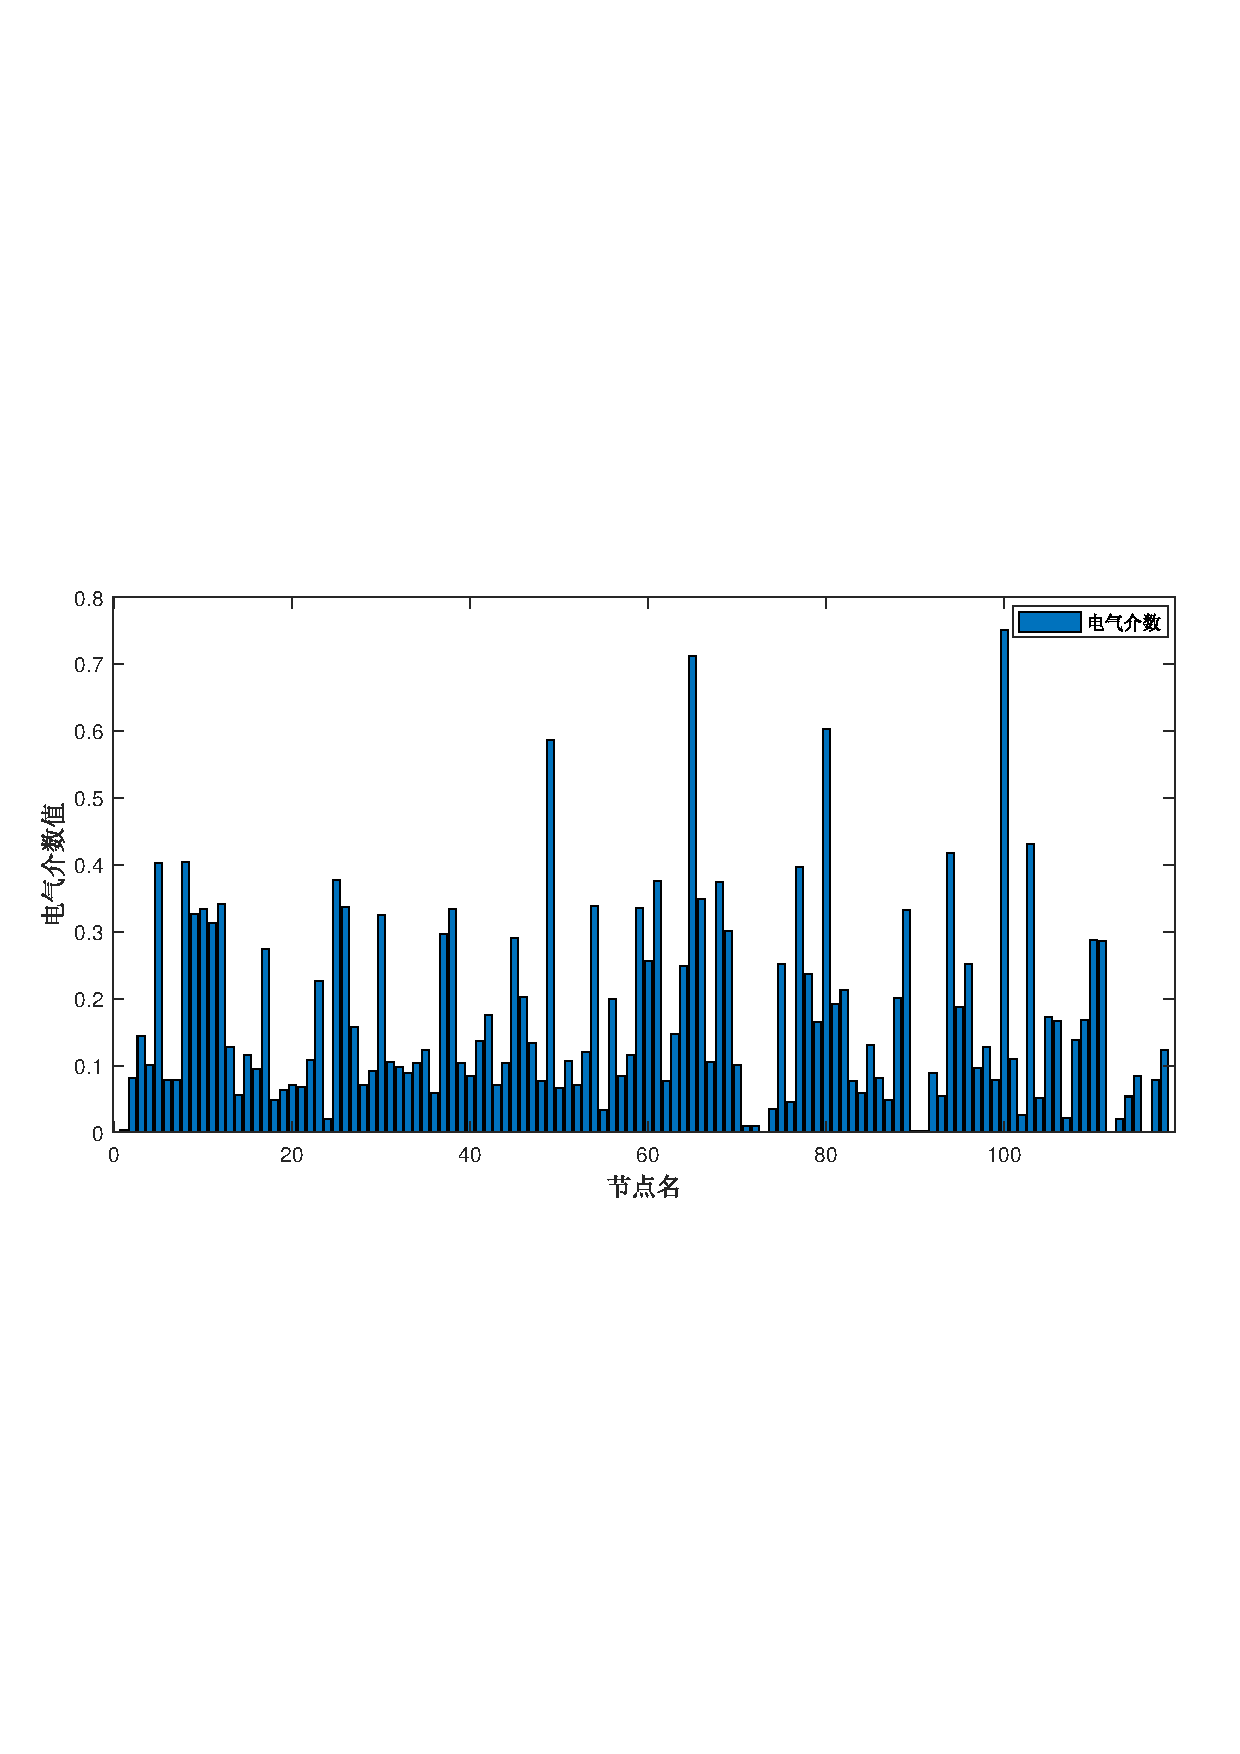
\includegraphics[width=14cm,height=7cm]{nodebetween118.pdf}
    \caption{$IEEE118$节点电气介数计算结果图}
    \label{fig:nodeBetween118}
\end{figure}
\begin{figure}[H] % use float package if you want it here
    \centering
    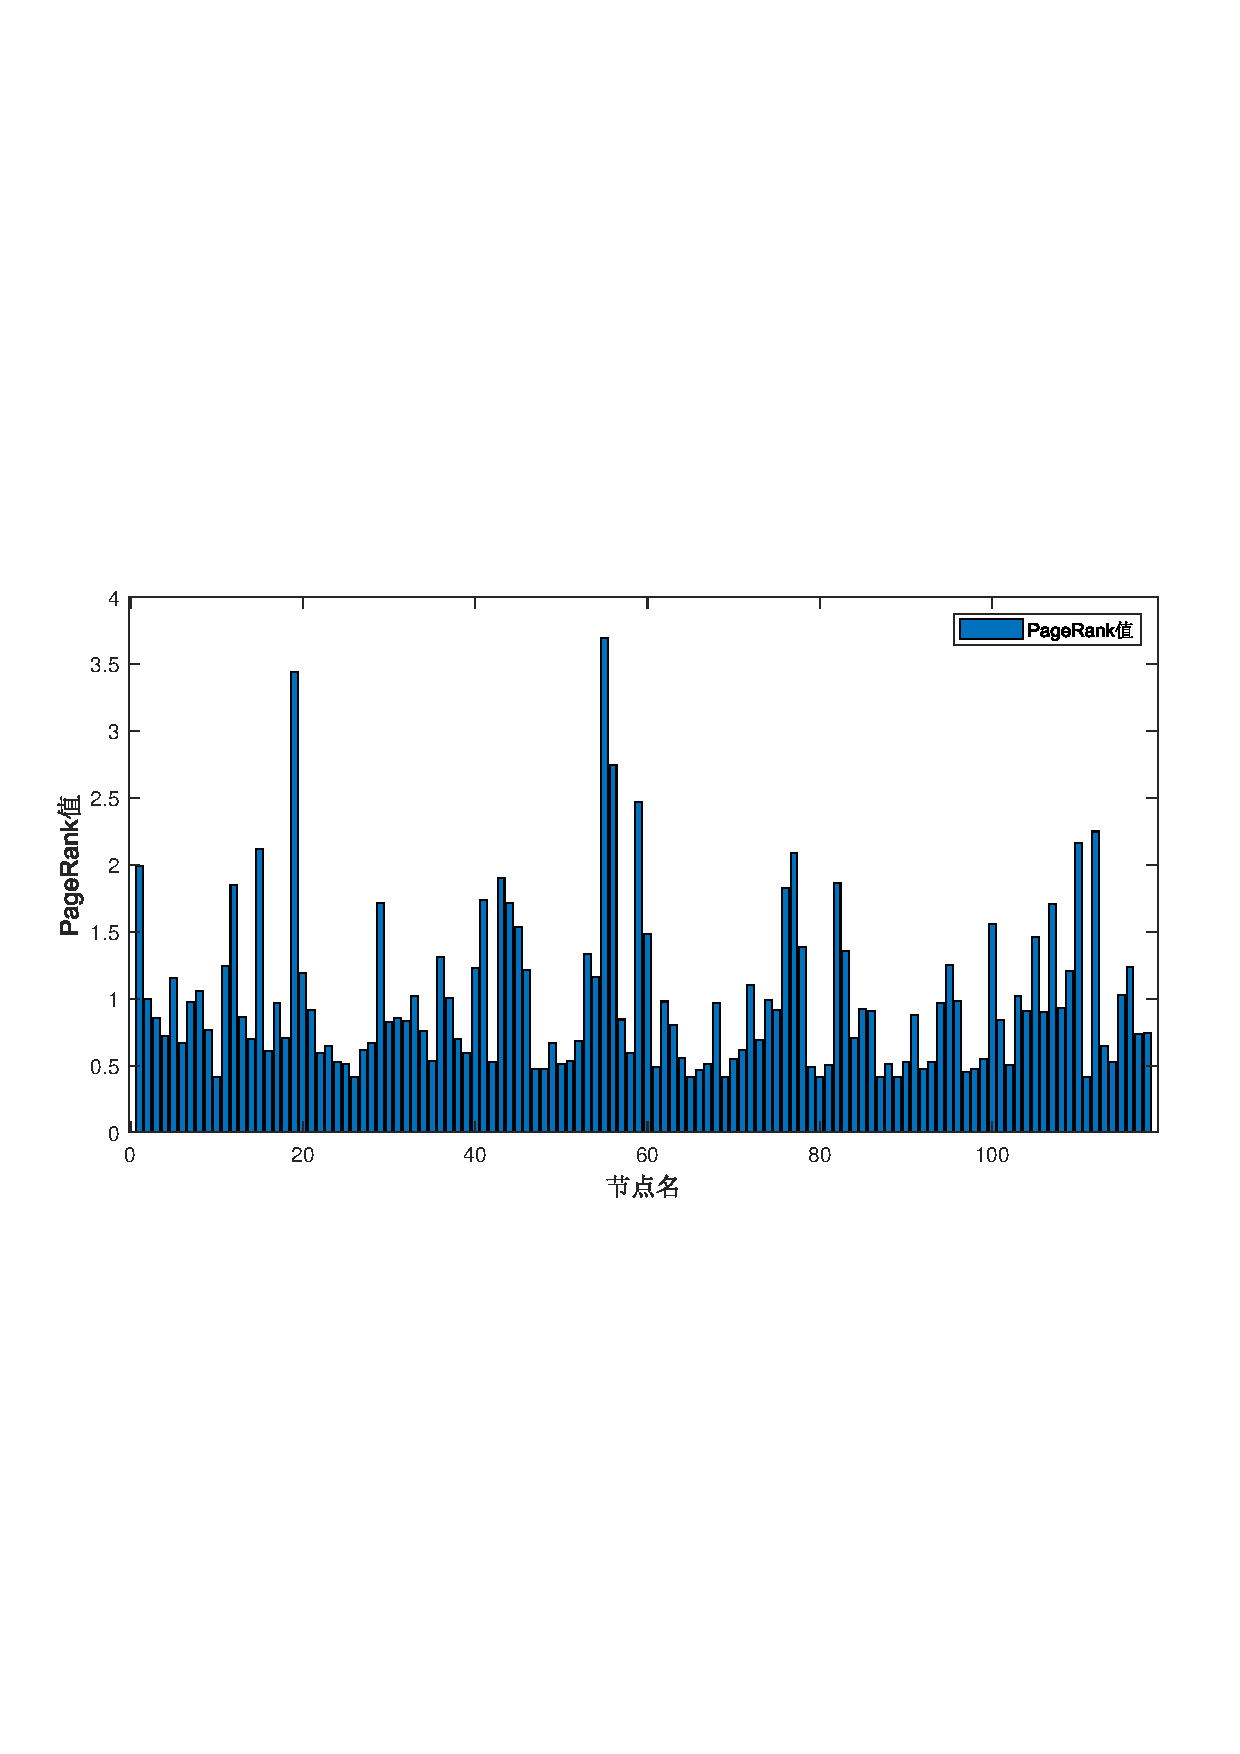
\includegraphics[width=14cm,height=7cm]{PageRank118.pdf}
    \caption{$IEEE118$节点PageRank值计算结果图}
    \label{fig:pagerank118}
\end{figure}

从图\ref{fig:electricDu118}、\ref{fig:nodeBetween118}和\ref{fig:pagerank118}可以看出,电气度指标值较高的节点名有9、8、49、5、30、89等,这些节点在电网结构中的邻接节点较多,
所连支路承担的潮流值较大;电气介数指标值较高的节点名有100、65、80、49、103等,表明电气介数值较大节点在结构和能量传输方面的重要程度高;PageRank指标值较高的节点名有1、55、19、56、59等,
这些节点的入链数目多,在潮流累计分布中比重较大。因此,在电网结构中的重要程度高。

下面为电气度、电气介数、$PageRank$值按照重要程度的节点号排名,取移除比例为$30\%$的节点数量。如表\ref{tab:rank118}所示。
\begin{table}[H]
    \centering
    \caption{电气度、电气介数、$PageRank$值节点号排名}
    \label{tab:rank118}
      \begin{tabular}{C{3cm}C{3cm}C{3cm}C{4cm}}
        \toprule
        节点排名  & 电气度节点名   & 电气介数节点名     & PageRank值节点名\\
        \midrule
        1       & 9              & 100                & 1 \\
        2       & 8              & 65                 & 55 \\
        3       & 49             & 80                 & 19 \\
        4       & 5              & 49                 & 56 \\
        5       & 30             & 103                 & 59 \\
        6       & 89             & 94                 & 112 \\
        7       & 69             & 8                 & 110 \\
        8       & 37             & 5                 & 15 \\
        9       & 38             & 77                 & 77 \\
        10      & 65             & 25                 & 43 \\
        11      & 17               & 61                & 82 \\
        12      & 92               & 68                 & 12 \\
        13      & 80               & 12                 & 76 \\
        14      & 10                 & 54                 & 41 \\
        15      & 68                 & 26                 & 44 \\
        16      & 66                 & 59                 & 29 \\
        17      & 25                 & 10                 & 107 \\
        18      & 64                 & 38                 & 100 \\
        19      & 77                 & 89                 & 45 \\
        20      & 59                 & 9                 & 60 \\
        21      & 100                & 30                 & 105 \\
        22      & 63                 & 11                 & 78 \\
        23      & 23                 & 69                 & 83 \\
        24      & 26                 & 37                 & 53 \\
        25      & 103                & 45                 & 36 \\
        26      & 75                 & 110                 & 95 \\
        27      & 85                 & 111                 & 11 \\
        28      & 11                 & 17                 & 116 \\
        29      & 61                 & 60                 & 40 \\
        30      & 27                 & 75                 & 46 \\
        31      & 94                 & 96                 & 109 \\
        32      & 116                 & 64                 & 20 \\
        33      & 110                 & 78                 & 54 \\
        34      & 90                 & 23                 & 5 \\
        35      & 4                 & 82                 & 72 \\
        36      & 12                 & 46                 & 8 \\
        37      & 60                & 88                 & 115 \\
        38      & 70                 & 56                 & 33 \\
        39      & 42                & 81                 & 103 \\
        \bottomrule
      \end{tabular}
\end{table}

下面为四种攻击策略下的仿真结果,如图\ref{fig:chap5:4Efficiency118}、\ref{fig:chap5:Efficiency118}所示。
\begin{figure}[H] % use float package if you want it here
  \centering
  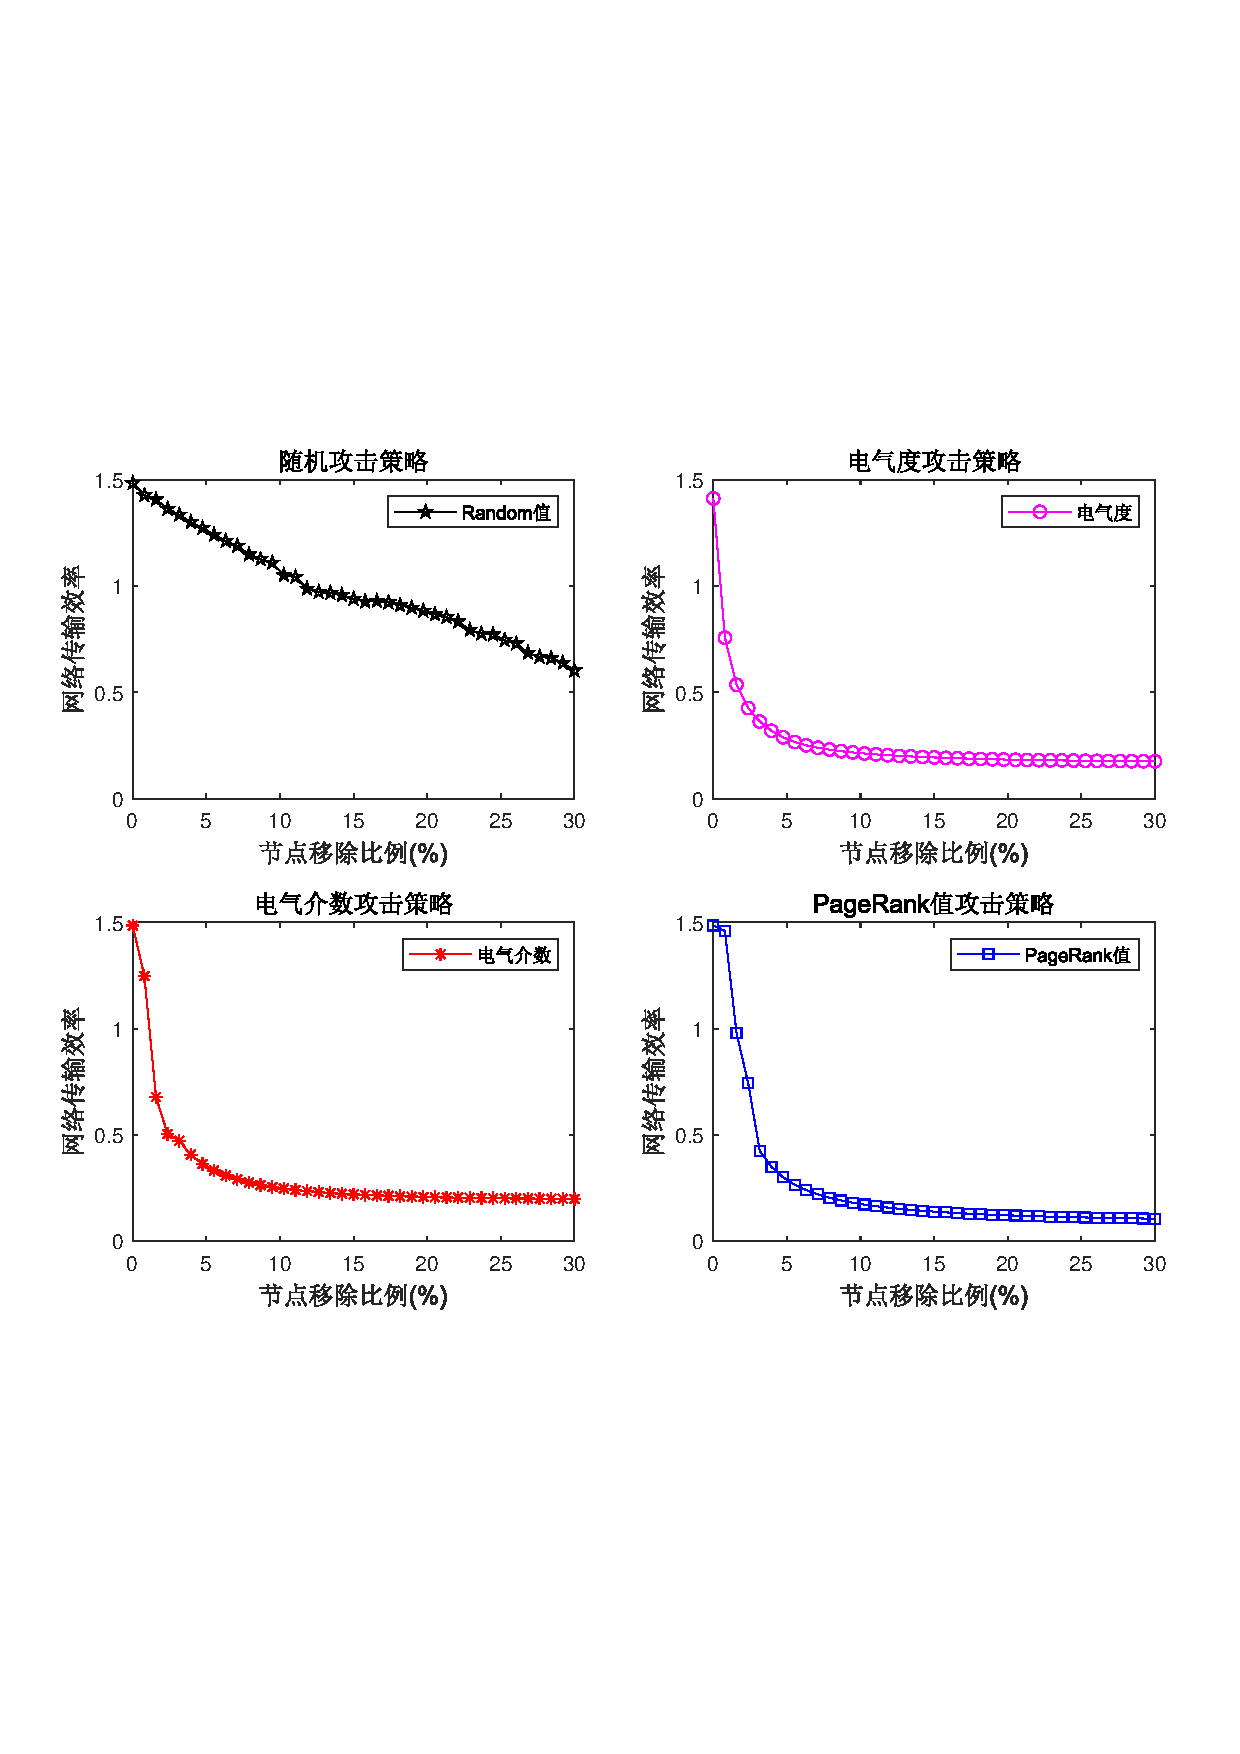
\includegraphics[width=13.4cm,height=9.6cm]{4Efficiency118.pdf}
  \caption{四种攻击策略下电网平均传输效率趋势图}
  \label{fig:chap5:4Efficiency118}
\end{figure}
\begin{figure}[H] % use float package if you want it here
  \centering
  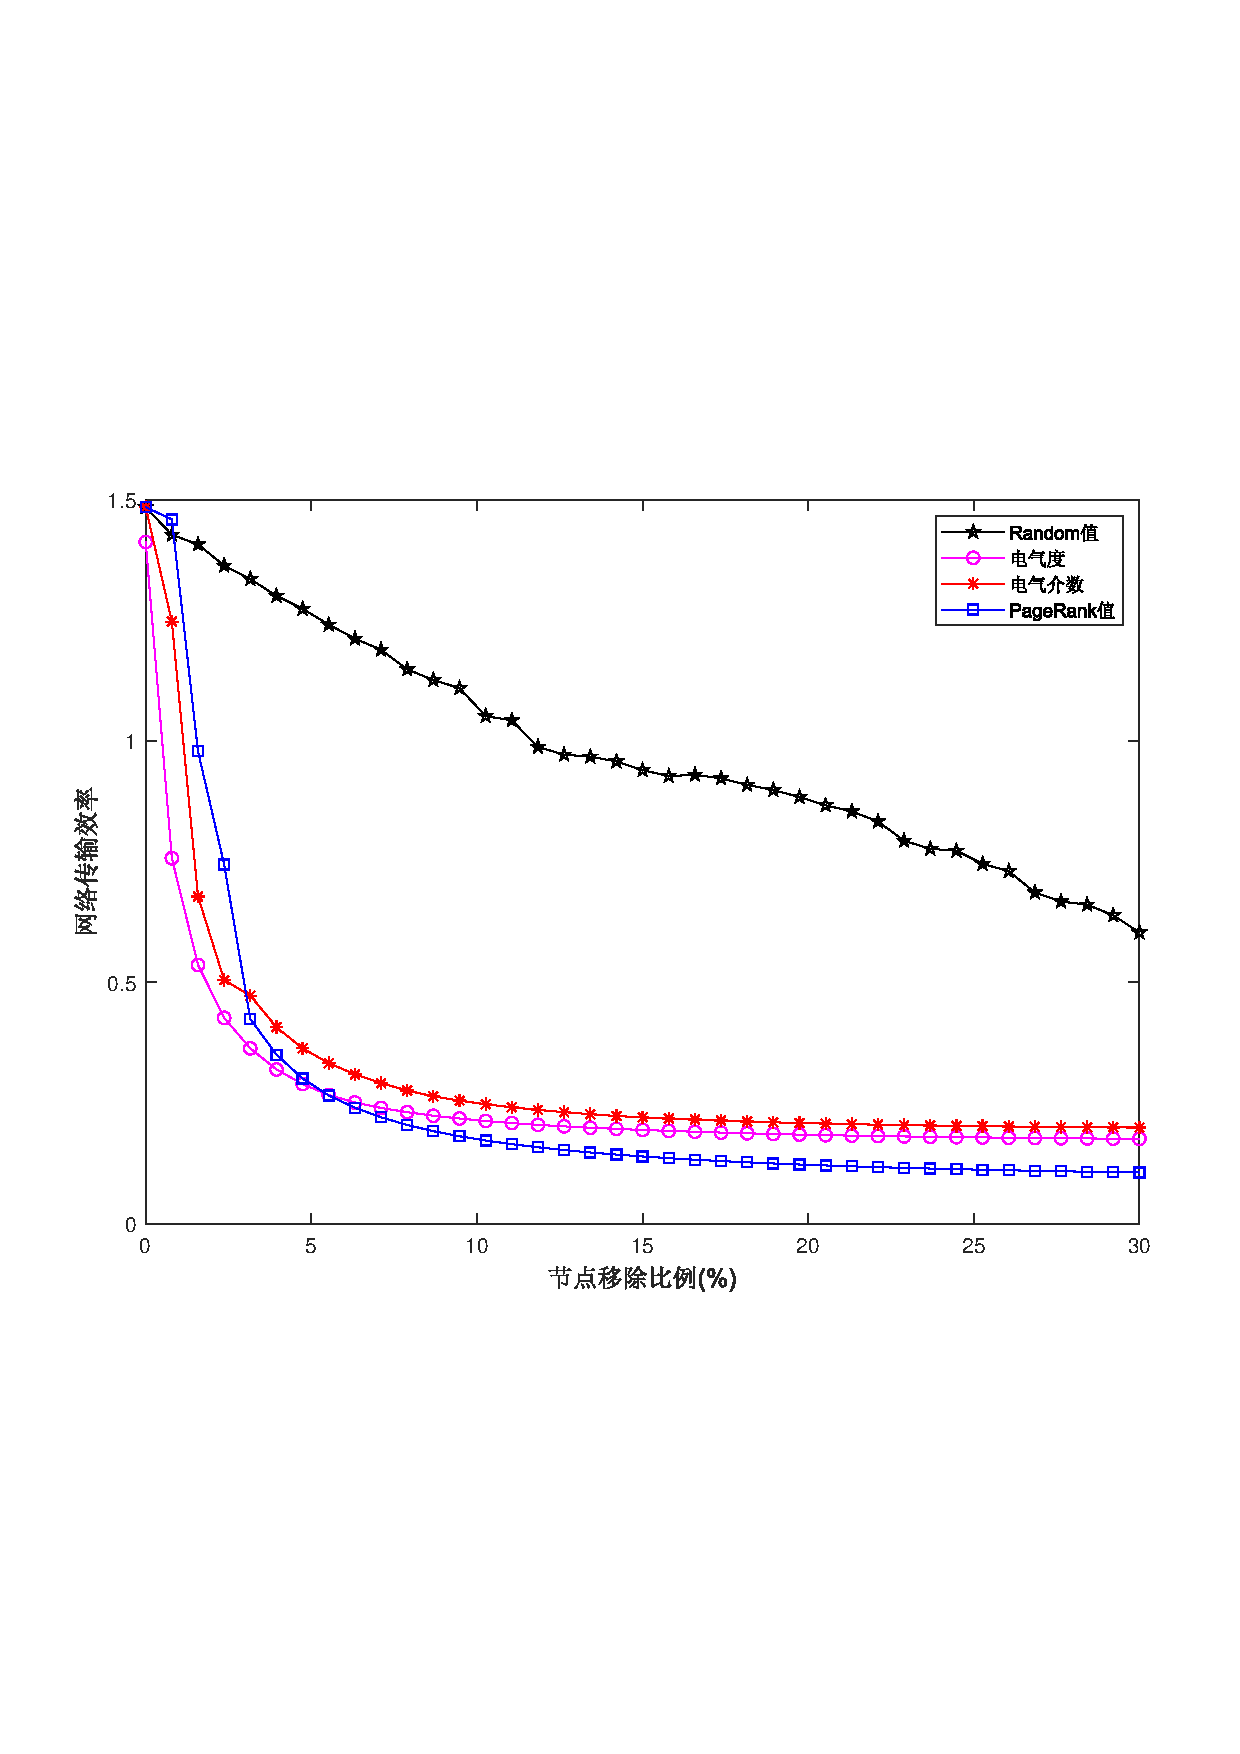
\includegraphics[width=13.4cm,height=9.1cm]{Efficiency118.pdf}
  \caption{四种电网攻击策略结果对比图}
  \label{fig:chap5:Efficiency118}
\end{figure}

从图\ref{fig:chap5:4Efficiency118}、\ref{fig:chap5:Efficiency118}的实验结果可以看出:

$(1)$在随机攻击策略下,网络传输效率值下降较为平缓,在节点移除比例至$30\%$时,电网的传输效率约为原来传输效率的$40\%$。而与其他三种攻击策略相比,
电气度、电气介数和$PageRank$值攻击策略对于电网传输效率的破坏性更高,在移除比例约为$10\%$时,电网平均传输效率已分别降至原来的$14.9\%$、$17.6\%$和$12.8\%$。因此,本文基于复杂网络
理论得到的脆弱性指标可以科学合理地描述系统各节点在电网中的重要程度,并可进一步衡量各节点在电网中的脆弱性。

$(2)$随机攻击策略对于电网的连通性影响较小,而蓄意攻击将会对网络连通性及传输效率影响较大,说明电网对于随机攻击具有很好的鲁棒性,进一步证实了电网的无标度性。

$(3)$对比三种蓄意攻击策略,从图\ref{fig:chap5:Efficiency118}得到,在节点移除前期,电气度攻击对于电网平均传输效率下降趋势最为明显,其原因在于,电气度是基于节点度进行定义的,电气度
指标更多的是专注于电网拓扑结构的重要性。在电气度的攻击策略下,节点的移除时意味着最大程度切断其他节点与所移除节点的联系,这将极大地破坏电网的拓扑结构,进而影响电网传输性能。可以证实,
电网拓扑结构的稳定性是电力系统正常运行的重要保证和前提条件,其节点的分布和联系是影响电网脆弱性的重要因素。在节点移除的后期,电气度、电气介数和$PageRank$值攻击策略对电网传输效率值分别
下降为$11.71\%$、$13.26\%$、$7.06\%$,在后期的移除过程中,$PageRank$值攻击策略的破坏性更高,原因在于,$PageRank$值指标关注的是潮流流向对于电网结构的重要性,指向节点的潮流数越多意味着
此节点的重要性越高,按照此攻击策略进行移除,将会导致发电节点所传输的功率所供给的节点越来越少,传输效率下降,直至无法进行功率传输。

综上分析,电气度、电气介数和$PageRank$的攻击策略相较于随机攻击策略的破坏性较大,从而验证了这三种指标可作为脆弱性指标的合理性。通过三种蓄意攻击策略的对比,可得到电气度专注于电网结构拓扑的
重要性,PageRank值则侧重于节点入链数的重要性,而电气介数综合考虑节点支路和支路潮流对电网结构的影响程度,其对电网的破坏性较为均衡。


\section{电力系统脆弱性分析评估}
\label{sec:singleAssessment}

本文基于$IEEE39$标准电网算例对电网脆弱性的研究工作,分别从结构和状态两个方面研究系统脆弱性,分析各系统节点对电网拓扑结构的影响程度,以及各节点对于电网故障及扰动的能力,最后将结构与状态
这两方面进行融合,综合评价系统的脆弱性,识别出电力系统的脆弱环节。

\subsection{电力系统结构脆弱性实验分析}
\label{sec:singleAnalysis_fabric}
本文选择的电网仿真模型为新英格兰测试系统数据——$IEEE39$,该系统由10个发电节点、29个负荷节点和46条支路组成。该系统的基准电压为345$KV$,基准功率为100$MVA$。
负荷节点序号为1-29;发电节点序号为30—39;31号节点为平衡节点。具体模型数据见附录A。

针对$IEEE39$标准算例系统的节点连接情况,可以得到如下的电网结构示意图。
\begin{figure}[H] % use float package if you want it here
  \centering
  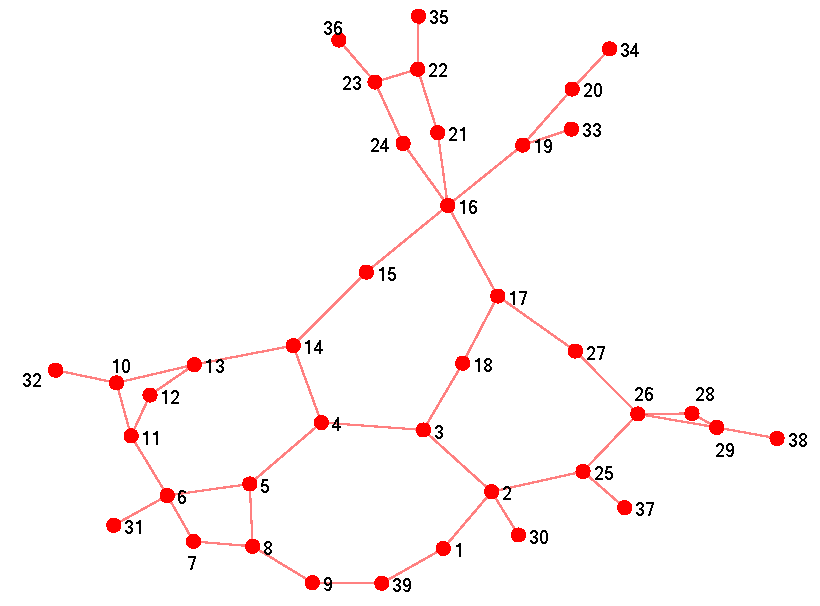
\includegraphics[height=7.5cm]{fabric_39.pdf}
  \caption{$IEEE39$系统拓扑示意图}
  \label{fig:fabric_39}
\end{figure}

\begin{figure}[H] % use float package if you want it here
  \centering
  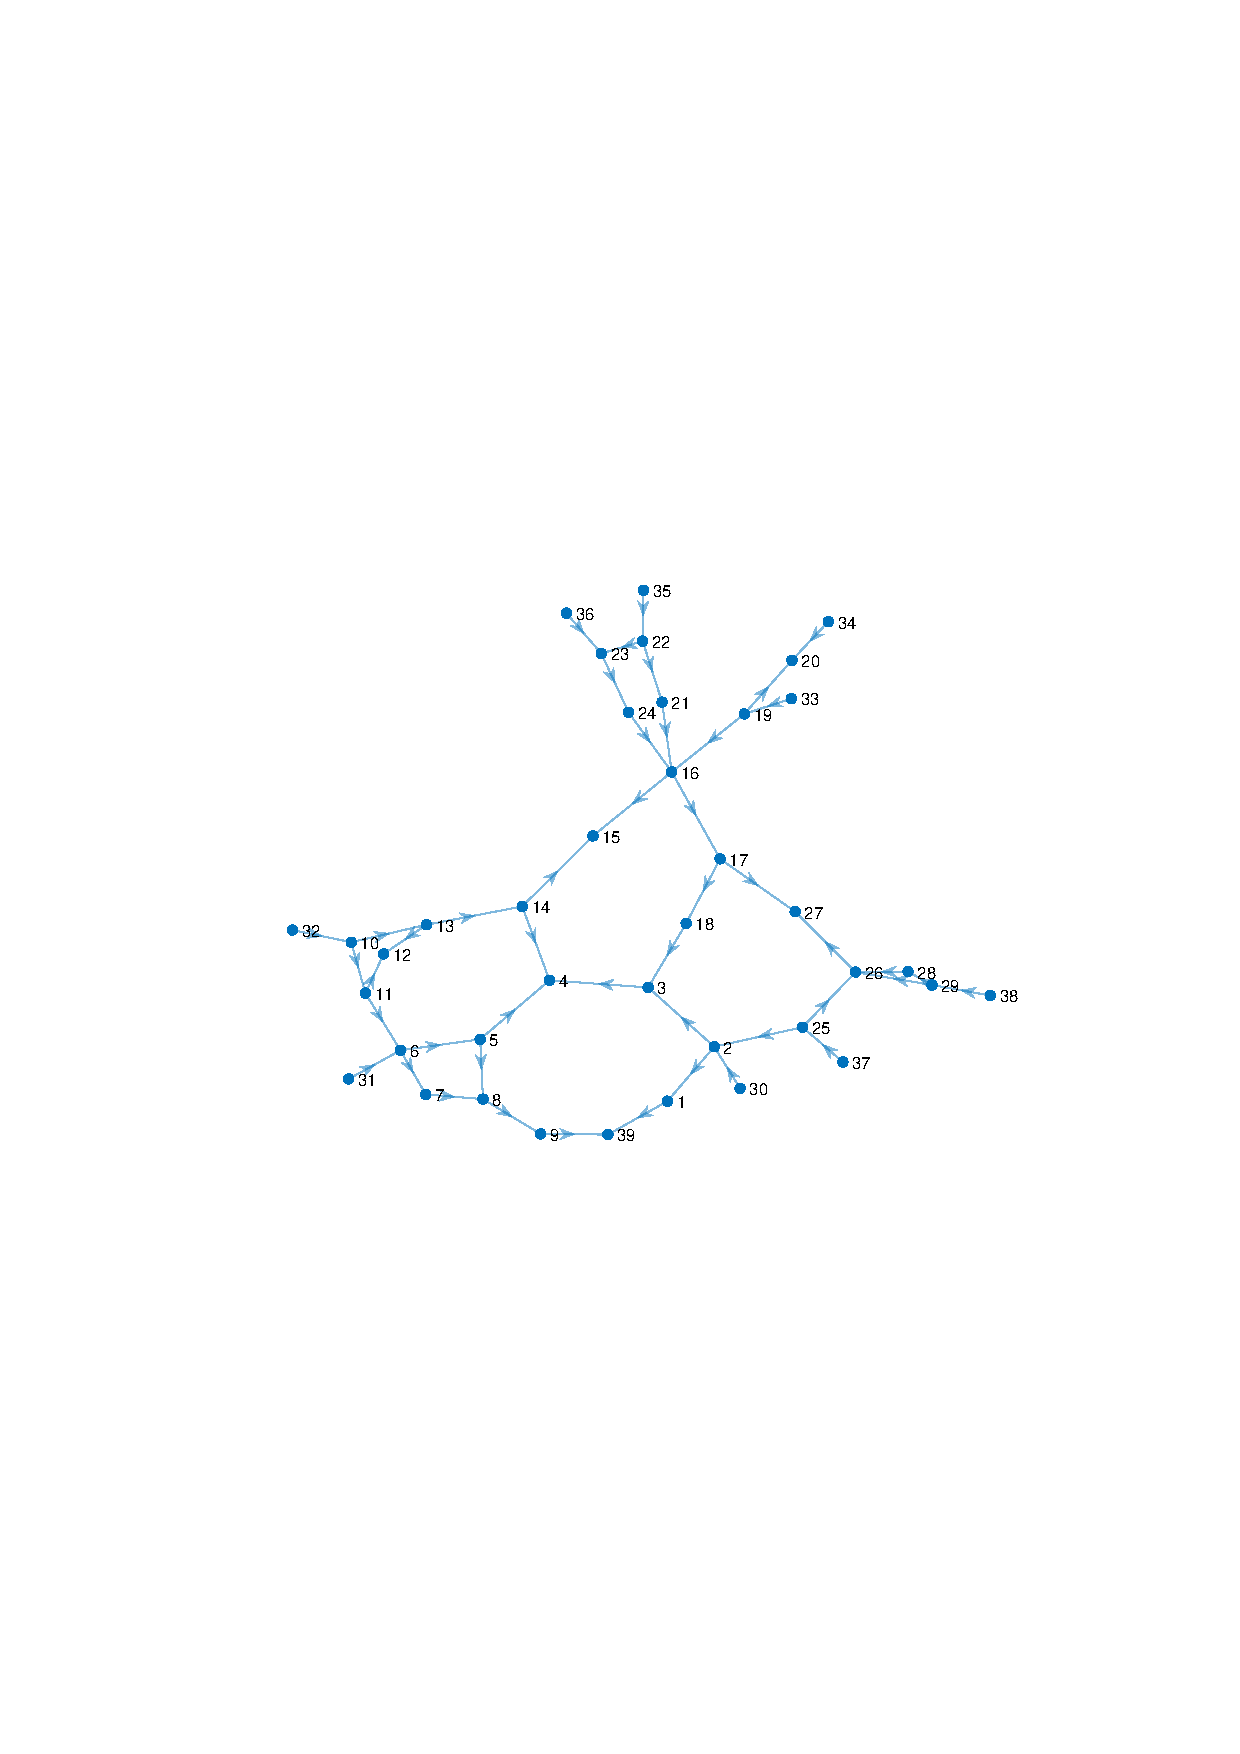
\includegraphics[height=8cm]{PageRank_39.pdf}
  \caption{$IEEE39$系统潮流有向图}
  \label{fig:PageRank_39}
\end{figure}


电气度、电气介数和PageRank值是基于复杂网络理论从不同的角度提出的结构脆弱性评价指标,为了不改变指标数据的原始分布,充分反映的是系统各节点在结构中的重要程度,对于结构脆弱性指标采用离散标准化的
归一化方法,得到各结构脆弱性指标数据后,采用改进的熵权法对电气度、电气介数和PageRank值这三个指标进行权重分配,得到权重向量$W_1 = \left[w_{1}\ w_{2}\ w_{3}\right]=[0.33\ 0.41\ 0.26]$,
并融合得到结构综合脆弱性指标。如表\ref{tab:chap5:Index_frabric39}所示。
\begin{table}[H]
  \centering
  \caption{IEEE39~系统结构脆弱性指标}
  \label{tab:chap5:Index_frabric39}
  \begin{tabular}{C{1.5cm}C{2.75cm}C{2.75cm}C{3.25cm}C{2.75cm}}
  \toprule
  \textbf{节点序号} & \textbf{电气度指标} & \textbf{电气介数指标} & \textbf{PageRank值指标} & \textbf{结构综合脆弱性指标} \\
  \midrule
  1 & 0.086924952 & 0.230348929 & 0.131020681 & 0.157193672 \\ 
  2 & 0.507756514 & 0.713870587 & 0.298554703 & 0.537870813 \\ 
  3 & 0.212417624 & 0.711647114 & 0.639183338 & 0.528060801 \\ 
  4 & 0.260485416 & 0.572099497 & 1           & 0.580520981 \\ 
  5 & 0.518219694 & 0.226085642 & 0.209128679 & 0.318081069 \\ 
  6 & 1           & 0.503485706 & 0.314075081 & 0.61808866 \\
  7 & 0.309635969 & 0.277191576 & 0.179009284 & 0.26237083 \\ 
  8 & 0.319050739 & 0.608998063 & 0.462906823 & 0.475331724 \\ 
  9 & 0.047102245 & 0.451887203 & 0.514658016 & 0.334628578 \\ 
  10 & 0.644344321 & 0.690312667 & 0.121158521 & 0.527163035 \\ 
  11 & 0.321857272 & 0.424945152 & 0.114064772 & 0.310097253 \\ 
  12 & 0           & 0           & 0.052371565 & 0.013616607 \\
  13 & 0.313506292 & 0.252871293 & 0.110080368 & 0.235755202 \\ 
  14 & 0.294699744 & 0.244978418 & 0.187549614 & 0.246454967 \\ 
  15 & 0.150832887 & 0.380901879 & 0.508650374 & 0.33819372 \\ 
  16 & 0.702443253 & 1           & 0.782654015 & 0.845296317 \\ 
  17 & 0.203569872 & 0.207053465 & 0.332121968 & 0.23842169 \\ 
  18 & 0.08070881  & 0.182479179 & 0.32250596  & 0.18530192 \\ 
  19 & 0.613414417 & 0.676656584 & 0.121158521 & 0.511357172 \\ 
  20 & 0.316762885 & 0.692736421 & 0.183458526 & 0.436252901 \\ 
  21 & 0.445971669 & 0.664135765 & 0.204129549 & 0.472539997 \\ 
  22 & 0.653758374 & 0.687089744 & 0.121158521 & 0.528948274 \\ 
  23 & 0.462785664 & 0.693184789 & 0.141174112 & 0.473630302 \\ 
  24 & 0.194520487 & 0.383108926 & 0.241158154 & 0.28396754 \\ 
  25 & 0.408317466 & 0.66937866  & 0.121158521 & 0.44069123 \\ 
  26 & 0.303558847 & 0.402464484 & 0.370358706 & 0.361478121 \\ 
  27 & 0.119219078 & 0.33135194  & 0.516940852 & 0.309601212 \\ 
  28 & 0.210788875 & 0.25769646  & 0.144614587 & 0.21281567 \\ 
  29 & 0.670307453 & 0.683970816 & 0.121158521 & 0.53313071 \\ 
  30 & 0.105556919 & 0.510686205 & 0           & 0.244215127 \\ 
  31 & 0.306737872 & 0.026491918 & 0           & 0.112085184 \\ 
  32 & 0.29880342  & 0.690312667 & 0           & 0.381633322 \\ 
  33 & 0.283977411 & 0.68455485  & 0           & 0.374380034 \\ 
  34 & 0.22519754  & 0.665173423 & 0           & 0.347036292 \\ 
  35 & 0.302835147 & 0.690312667 & 0           & 0.382963792 \\ 
  36 & 0.246277315 & 0.676175494 & 0           & 0.358503467 \\ 
  37 & 0.237532647 & 0.673137612 & 0           & 0.354372194 \\ 
  38 & 0.387392146 & 0.690559802 & 0           & 0.410968927 \\ 
  39 & 0.015510059 & 0.695379301 & 0.791086603 & 0.49590635 \\ 
  \bottomrule
  \end{tabular}
\end{table}
在$IEEE39$系统中,电气度指标值最大的为节点6,最小的为节点12;电气介数指标值最大的为节点16,最小的为节点12;PageRank值最大的为节点4,最小的为发电节点30、31、32、33、34、35、36、37、38。
在基于PageRank的$IEEE39$拓扑模型中,发电节点30—38无入链数,并且其出链数均为1,所以其PageRank值相同且最小。对于节点12,从表中可以看出,其电气度和电气介数指标值均最小,从$IEEE39$电网结构
拓扑图中可以看出节点12与节点11和节点13连接,与其他节点相比节点度较小,根据附录A$IEEE39$系统数据,其功率容量较小,并且节点11和节点13均为联络节点(无功率容量),这导致节点12所连接支路的
视在功率较小,从而计算得到的电气度指标值较小。节点电气介数综合结构和潮流能量进行定义,该指标值与支路和节点的有功功率容量正相关,因此,在IEEE39系统中,节点12的电气介数值最小。节点6和16在
节点度和支路潮流值上,较其他节点都比较大,因此,根据电气度和电气介数的计算方法,其指标数值最大。

根据权重向量计算得到的系统结构综合脆弱性指标结果如图~\ref{fig:stric_39}~所示。
\begin{figure}[H] % use float package if you want it here
  \centering
  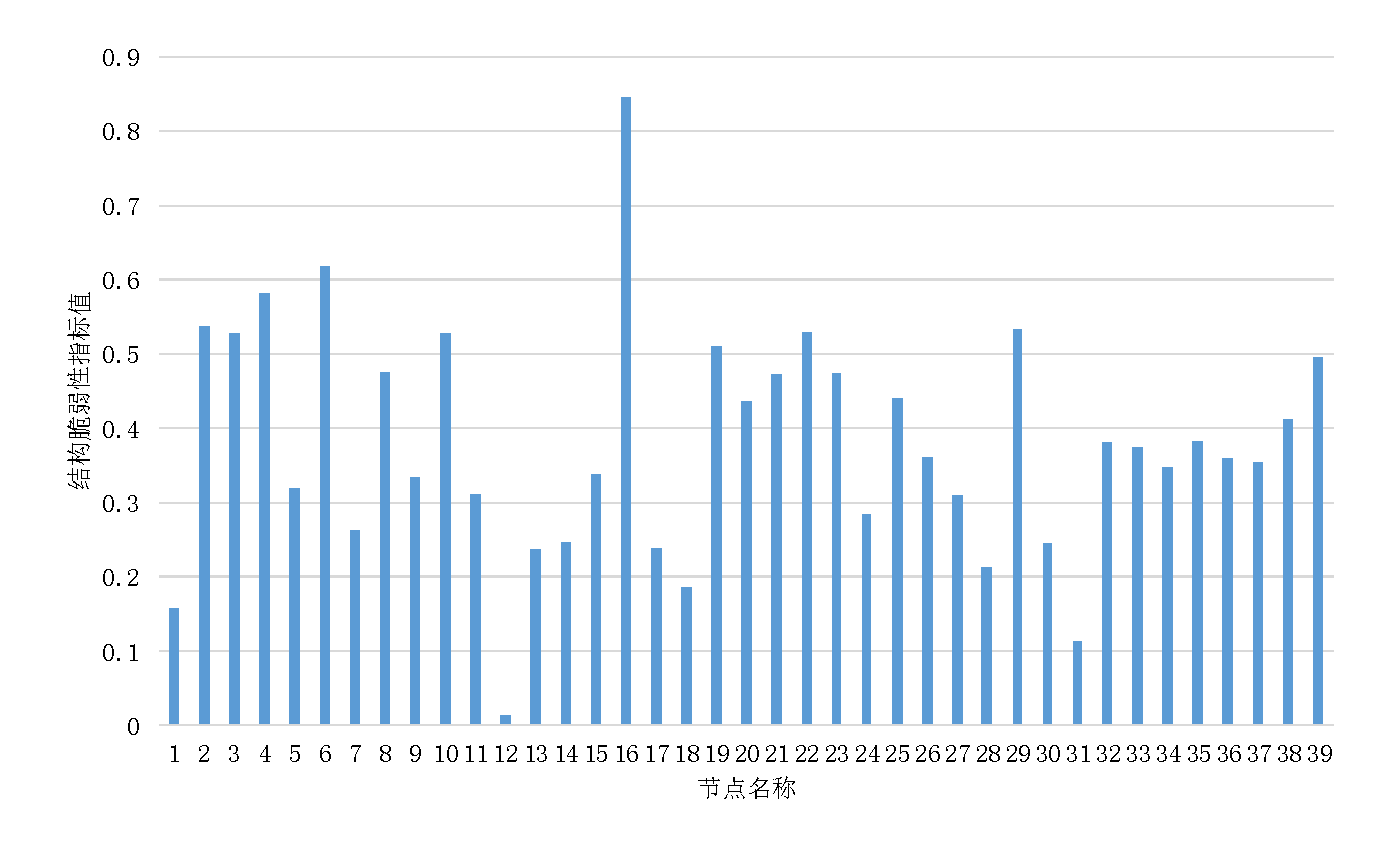
\includegraphics[width=14cm,height=8.64cm]{stric_39.pdf}
  \caption{IEEE39结构综合脆弱性指标}
  \label{fig:stric_39}
\end{figure}

从图~\ref{fig:stric_39}~可知,系统结构综合脆弱性最高的节点是16。从表~\ref{tab:chap5:Index_frabric39}~其在电气度、电气介数和PageRank值中的指标数值分别为0.7、1和0.78,从这
三个指标角度考虑来看,节点16在此系统结构的重要程度较高。从结构示意图不难看出,节点16位于系统结构的中心位置,与其连接的有15、17、19、21和24节点,综合图\ref{fig:PageRank_39}来看,
节点16的入链数3条,出链数2条,较其他节点而言,节点16所连支路承担着较多的能量传输,假设节点16发生故障,$IEEE39$电网系统会随即裂解成三个子网络,从而影响电网网运行。节点2、4、6、
10、29的重要性也比较高,从节点位置可以看出,这些节点大都连接发电节点,如节点30、31、32、38,承担着将发电节点产生的能量传送至各负荷节点,支路潮流值较大。因此,这些节点不论从节点
连接情况和潮流分布情况而言对于系统结构起到重要作用,所以这些节点的结构综合脆弱程度高。另一方面,节点12、31、1、18、28的结构综合脆弱性指标值较小,所连节点一般为联络节点或容量较小的负荷节点,
其节点节点容量潮流累计和支路潮流值较小,假设这些节点发生故障,并不会对系统结构的完整性造成较大的影响,因此,这些节点的结构位置在系统中的作用较小,所连支路对于电能的传输能力也较小,
故其结构综合脆弱程度低。

\subsection{电力系统状态脆弱性实验分析}
\label{sec:singleAnalysis_status}
在状态脆弱性指标集中,本文通过模拟实际电网负荷变化,通过潮流计算得到电压稳定裕度指标值,采用第三章所建立的正态分布负荷模型中,如式\ref{equ:chap3:probability}所示,其中均值$\mu$设置为
对应负荷节点的额定功率,标准差$\sigma$为负荷节点额定功率的$0.2$倍,所以电网负荷模型负荷功率95.45$\%$分布在额定功率的0.8到1,2倍之间,并通过蒙特卡洛模拟实验进行仿真,仿真次数为10000,
以式\ref{equ:chap3:SV}进行计算,取平均值作为最终结果;在功率裕度指标计算中,式\ref{equ:chap3:SC}中,最大负荷功率依据式\ref{equ:chap3:probability1}通过连续潮流计算得到,其中$Q_{target}$
设置为1.5倍的额定功率;在电网损耗灵敏度指标计算中,每个负荷节点在额定负荷$\pm 10 \%$范围内取100个计算点进行潮流计算,所以步长设置为负荷节点0.002倍的额定功率。
根据系统节点各状态脆弱性指标值结果,基于最大离差化法得到权重向量$W_2 = \left[w_{1}\ w_{2}\ w_{3}\right]=[0.29\ 0.34\ 0.37]$并融合得到结构综合脆弱性指标。
如表\ref{tab:chap5:Index1_frabric39}所示。由于状态脆弱性指标集均基于负荷模型进行仿真实验,故在状态脆弱性研究时仅针对负荷节点进行分析,

\begin{table}[H]
  \centering
  \caption{IEEE39~系统状态脆弱性指标}
  \label{tab:chap5:Index1_frabric39}
  \begin{tabular}{C{1.5cm}C{2.75cm}C{2.75cm}C{3.25cm}C{2.75cm}}
  \toprule
  \textbf{节点序号} & \textbf{电压裕度指标} & \textbf{功率裕度指标} & \textbf{电网损耗灵敏度指标} & \textbf{状态脆弱性指标} \\
  \midrule
  1 & 0 & 0.143529412 & 0.333864456 & 0.166619797 \\ 
  2 & 0.627763605 & 0 & 0 & 0.182051445 \\ 
  3 & 0.868532753 & 0.473529412 & 0.173992035 & 0.486237673 \\ 
  4 & 0.681365198 & 0.735294118 & 0.175148734 & 0.5292053 \\ 
  5 & 0.548173985 & 0 & 0 & 0.158970456 \\ 
  6 & 0.513990896 & 0 & 0 & 0.14905736 \\ 
  7 & 0.493134944 & 0.343823529 & 0.187816277 & 0.334081374 \\ 
  8 & 0.440628844 & 0.767647059 & 0.243415763 & 0.494573136 \\ 
  9 & 0.234327507 & 0.009558824 & 0.318257774 & 0.179699385 \\ 
  10 & 0.615287695 & 0 & 0 & 0.178433432 \\ 
  11 & 0.585145902 & 0 & 0 & 0.169692312 \\ 
  12 & 0.52049683 & 0.012544118 & 0.113091151 & 0.194036395 \\
  13 & 0.64839947 & 0 & 0 & 0.188035846 \\ 
  14 & 0.742688646 & 0 & 0 & 0.215379707 \\
  15 & 0.643616556 & 0.470588235 & 0.04447175 & 0.375886843 \\ 
  16 & 0.69500044 & 0.483823529 & 0.106956156 & 0.416929927 \\ 
  17 & 0.831020315 & 0 & 0 & 0.240995891 \\
  18 & 0.885074662 & 0.232352941 & 0.0783821 & 0.369292154 \\ 
  19 & 1 & 0 & 0 & 0.29 \\ 
  20 & 0.221686653 & 1 & 0.413774827 & 0.57497257 \\ 
  21 & 0.473735759 & 0.402941176 & 0.256847857 & 0.373799877 \\ 
  22 & 0.411534686 & 0 & 0 & 0.119345059 \\ 
  23 & 0.345775724 & 0.363970588 & 0.509079018 & 0.408030944 \\ 
  24 & 0.622365665 & 0.453823529 & 0.111699933 & 0.386378726 \\ 
  25 & 0.460615009 & 0.329411765 & 0.776181665 & 0.519362472 \\ 
  26 & 0.748966045 & 0.204411765 & 0.443079199 & 0.443479434 \\ 
  27 & 0.657596651 & 0.413235294 & 0.150193042 & 0.394665722 \\ 
  28 & 0.490373345 & 0.302941176 & 0.753896625 & 0.510621358 \\ 
  29 & 0.588829917 & 0.416911765 & 1 & 0.665018029 \\ 
  \bottomrule
  \end{tabular}
\end{table}

由于节点2、5、6、10、11、13、14、17、19和22为联络节点,其注入有功功率和无功功率都等于零,所以其负荷模型的数据为0,因此,在功率稳定裕度指标和电网损耗灵敏度指标中,将这些节点的指标数值设置为0。

根据权重向量计算得到的系统状态综合脆弱性指标结果如图~\ref{fig:state_39}~所示。
\begin{figure}[H] % use float package if you want it here
  \centering
  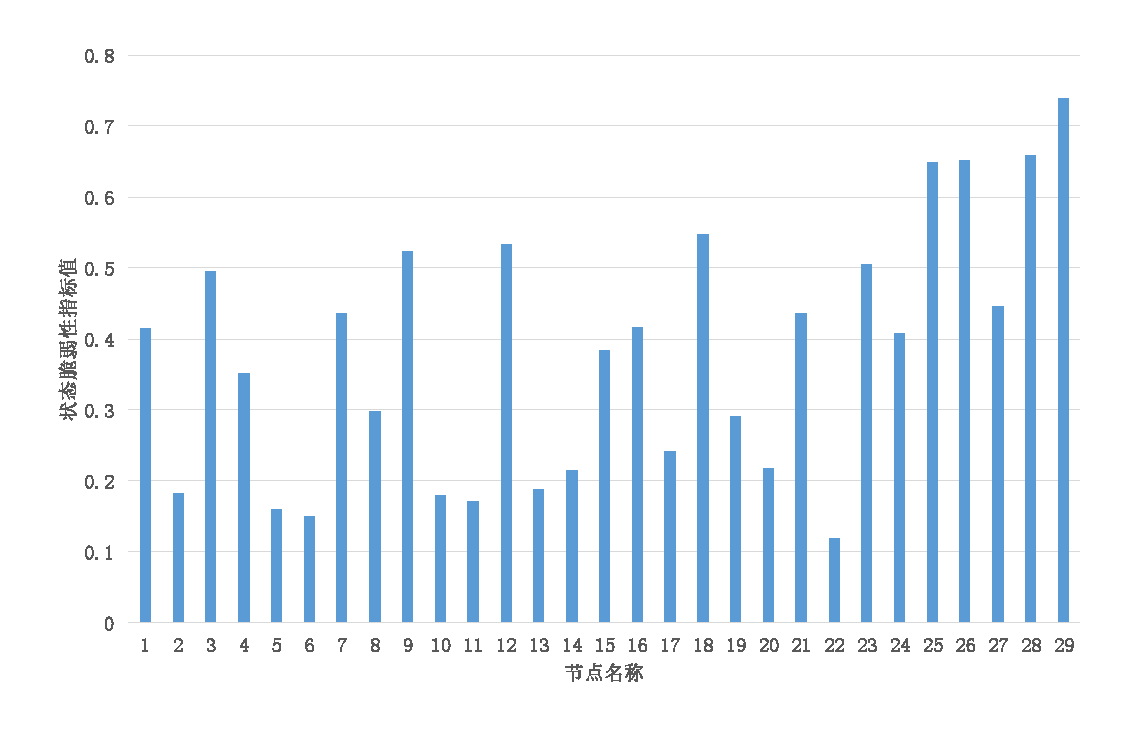
\includegraphics[width=14cm,height=8.64cm]{state_39.pdf}
  \caption{IEEE39状态综合脆弱性指标}
  \label{fig:state_39}
\end{figure}



\subsection{电力系统综合脆弱性分析}
\label{sec:singleAnalysis}





\section{电力系统脆弱性等级评估}
\label{sec:multiAssessment}




\subsection{基于聚类算法的电力系统脆弱等级评估}
\label{sec:multiVSsingle}




\subsection{基于综合指标排序的电力系统脆弱等级评估}
\label{sec:multiAnalysis}





\subsection{结果分析与比较}




\section{本章小结}
\label{sec:sum5}


